% Options for packages loaded elsewhere
\PassOptionsToPackage{unicode}{hyperref}
\PassOptionsToPackage{hyphens}{url}
\PassOptionsToPackage{dvipsnames,svgnames,x11names}{xcolor}
%
\documentclass[
  10pt,
]{article}
\usepackage{amsmath,amssymb}
\usepackage{iftex}
\ifPDFTeX
  \usepackage[T1]{fontenc}
  \usepackage[utf8]{inputenc}
  \usepackage{textcomp} % provide euro and other symbols
\else % if luatex or xetex
  \usepackage{unicode-math} % this also loads fontspec
  \defaultfontfeatures{Scale=MatchLowercase}
  \defaultfontfeatures[\rmfamily]{Ligatures=TeX,Scale=1}
\fi
\usepackage{lmodern}
\ifPDFTeX\else
  % xetex/luatex font selection
  \setmainfont[]{DejaVu Serif}
  \setmonofont[]{DejaVu Sans Mono}
\fi
% Use upquote if available, for straight quotes in verbatim environments
\IfFileExists{upquote.sty}{\usepackage{upquote}}{}
\IfFileExists{microtype.sty}{% use microtype if available
  \usepackage[]{microtype}
  \UseMicrotypeSet[protrusion]{basicmath} % disable protrusion for tt fonts
}{}
\makeatletter
\@ifundefined{KOMAClassName}{% if non-KOMA class
  \IfFileExists{parskip.sty}{%
    \usepackage{parskip}
  }{% else
    \setlength{\parindent}{0pt}
    \setlength{\parskip}{6pt plus 2pt minus 1pt}}
}{% if KOMA class
  \KOMAoptions{parskip=half}}
\makeatother
\usepackage{xcolor}
\usepackage[margin=18mm]{geometry}
\usepackage{longtable,booktabs,array}
\usepackage{calc} % for calculating minipage widths
% Correct order of tables after \paragraph or \subparagraph
\usepackage{etoolbox}
\makeatletter
\patchcmd\longtable{\par}{\if@noskipsec\mbox{}\fi\par}{}{}
\makeatother
% Allow footnotes in longtable head/foot
\IfFileExists{footnotehyper.sty}{\usepackage{footnotehyper}}{\usepackage{footnote}}
\makesavenoteenv{longtable}
\usepackage{graphicx}
\makeatletter
\def\maxwidth{\ifdim\Gin@nat@width>\linewidth\linewidth\else\Gin@nat@width\fi}
\def\maxheight{\ifdim\Gin@nat@height>\textheight\textheight\else\Gin@nat@height\fi}
\makeatother
% Scale images if necessary, so that they will not overflow the page
% margins by default, and it is still possible to overwrite the defaults
% using explicit options in \includegraphics[width, height, ...]{}
\setkeys{Gin}{width=\maxwidth,height=\maxheight,keepaspectratio}
% Set default figure placement to htbp
\makeatletter
\def\fps@figure{htbp}
\makeatother
\setlength{\emergencystretch}{3em} % prevent overfull lines
\providecommand{\tightlist}{%
  \setlength{\itemsep}{0pt}\setlength{\parskip}{0pt}}
\setcounter{secnumdepth}{-\maxdimen} % remove section numbering
\ifLuaTeX
  \usepackage{selnolig}  % disable illegal ligatures
\fi
\usepackage{bookmark}
\IfFileExists{xurl.sty}{\usepackage{xurl}}{} % add URL line breaks if available
\urlstyle{same}
\hypersetup{
  colorlinks=true,
  linkcolor={Maroon},
  filecolor={Maroon},
  citecolor={Blue},
  urlcolor={Blue},
  pdfcreator={LaTeX via pandoc}}

\author{}
\date{}

\begin{document}

\section{Complete cold costs and matched
compression}\label{complete-cold-costs-and-matched-compression}

\textbf{Status:} independently replayed finite software-count
diagnostic; benchmark admission remains incomplete.

The fixed plan contains 4749 profiles and 4749 attempted executions.
There are 60 distinct public DLP targets in this cohort. Configurations
and process repetitions are correlated; a recovered execution is not
another independent target.

\begin{longtable}[]{@{}lr@{}}
\toprule\noalign{}
Recorded cohort and outcome & Executions \\
\midrule\noalign{}
\endhead
\bottomrule\noalign{}
\endlastfoot
AA / recovered & 6 \\
archived-exhaustive-discovery / recovered & 3 \\
development-alpha / ambiguous & 12 \\
development-alpha / recovered & 360 \\
development-alpha / underfilled & 108 \\
development-cold / ambiguous & 408 \\
development-cold / recovered & 756 \\
development-cold / underfilled & 36 \\
development-reference / capped & 3 \\
development-reference / recovered & 897 \\
regression-60 / ambiguous & 1026 \\
regression-60 / recovered & 1134 \\
\end{longtable}

The ratios below use only successful matched recoveries, with every
unsuccessful attempt retained in the table above. Endpoints are observed
ranges, not confidence intervals.

\begin{longtable}[]{@{}
  >{\raggedright\arraybackslash}p{(\columnwidth - 2\tabcolsep) * \real{0.5000}}
  >{\raggedright\arraybackslash}p{(\columnwidth - 2\tabcolsep) * \real{0.5000}}@{}}
\toprule\noalign{}
\begin{minipage}[b]{\linewidth}\raggedright
Numerator / denominator
\end{minipage} & \begin{minipage}[b]{\linewidth}\raggedright
Median {[}min, max{]}; pairs
\end{minipage} \\
\midrule\noalign{}
\endhead
\bottomrule\noalign{}
\endlastfoot
Full / compressed, cold & 0.94084 {[}0.65134, 0.99974{]}, n=1125 \\
Full / compressed, matrix & 0.47265 {[}0.17979, 1.1047{]}, n=1848 \\
Ordinary / twist, cold & 0.98560 {[}0.55827, 1.2956{]}, n=750 \\
Map / scalar, cold & 0.99258 {[}0.98633, 0.99645{]}, n=180 \\
IC / strongest completed measured reference & 59.650 {[}7.3906,
8071.0{]}, n=2253 \\
\end{longtable}

Ratios below 1 favor the numerator. Compression cost more in every
successful matched cold pair in this implementation. The map/scalar
saving is available to ordinary bases too. The ordinary/twist ratios do
not establish a consistent twist-specific advantage. Five references
share each Q: native rho, negation/cycle-escape rho, BSGS, negation BSGS
and GP elllog. The strongest completed member is not a global
fastest-rho certificate.

The60-target collector regression has 720 matched groups. Group, native
full-root and GP full-root methods agree on the complete problem and
outcome. Three reference executions hit their fixed algorithm cap; they
are retained.

All raw instruction sums and completed source/map/full-fiber
computations pass independent native/GP checks. Initial GP references
were strictly rejected for undeclared automatic stack-growth warnings.
Their unchanged-script successors use a larger initial stack and pass
the same strict policy. No attack profile was repeated.

The original summary stopped on identical missing query hashes in
pre-query failures. A versioned post-data guard correction preserves
successful-pair eligibility and formulas. Both versions remain. The
pre-data machine protocol also encoded the explicit flat plan in fields
the canonical checker treats as a rectangular product. Export schema
checks pass, but full protocol/export admission fails (including the
analysis-source correction). These are descriptive diagnostics, not
promoted benchmark or leaderboard rows. The exact pre-data plan is
complete; the checker finding is not evidence of missing planned
profiles.

The unit is single-event guest instructions Ir, including actual
resident-GP instructions in each exclusive phase. Cold setup, queries,
complete decomposition, signs/deduplication, matrix work and
source-point verification are charged per target. Input/program loading
and result/trace serialization are excluded. No clock, cycle or
primitive/GAE conversion is used.

Conditional affine Lean lemmas retain their stated hypotheses. Concrete
arithmetic, rank/kernel spans and map fidelity are checked externally; a
fully formal concrete bridge is open. Literature and access gaps are in
the frozen protocol.

\newpage

\begin{figure}
\centering
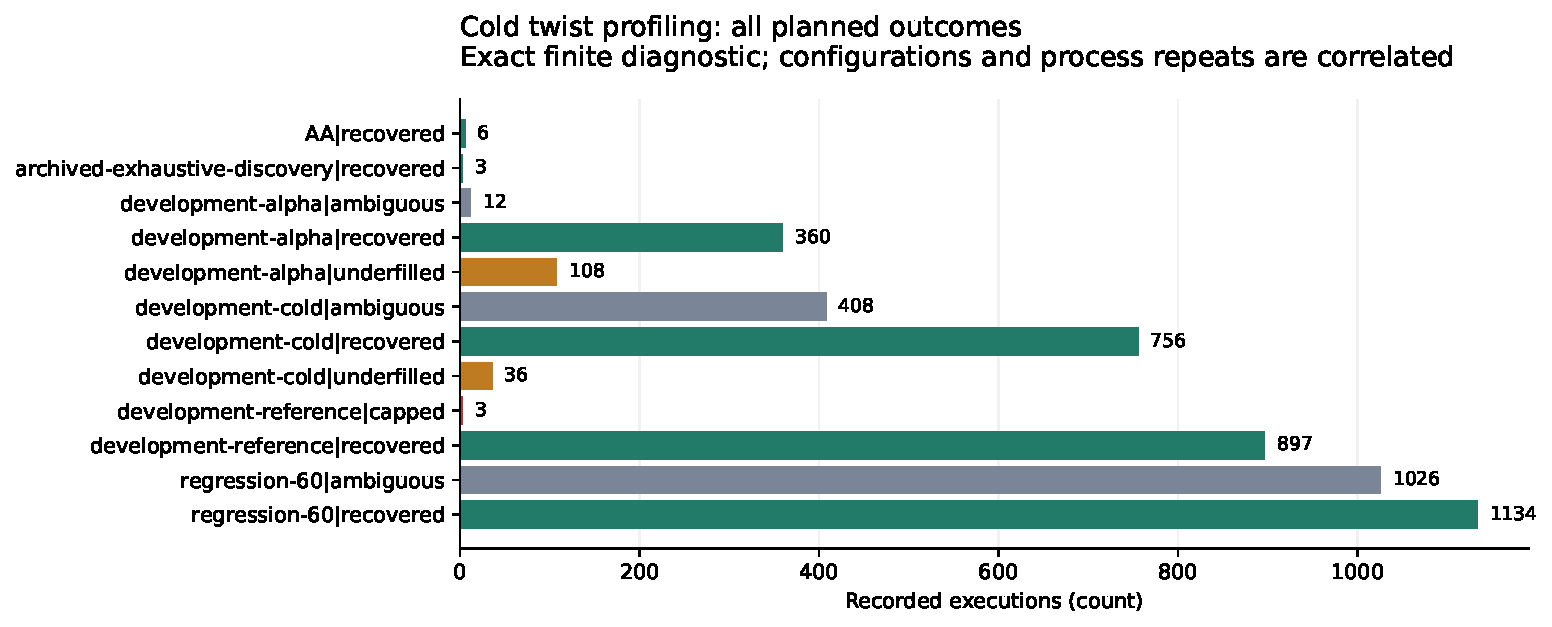
\includegraphics{OUTCOMES.pdf}
\caption{All recorded outcomes}
\end{figure}

\begin{figure}
\centering
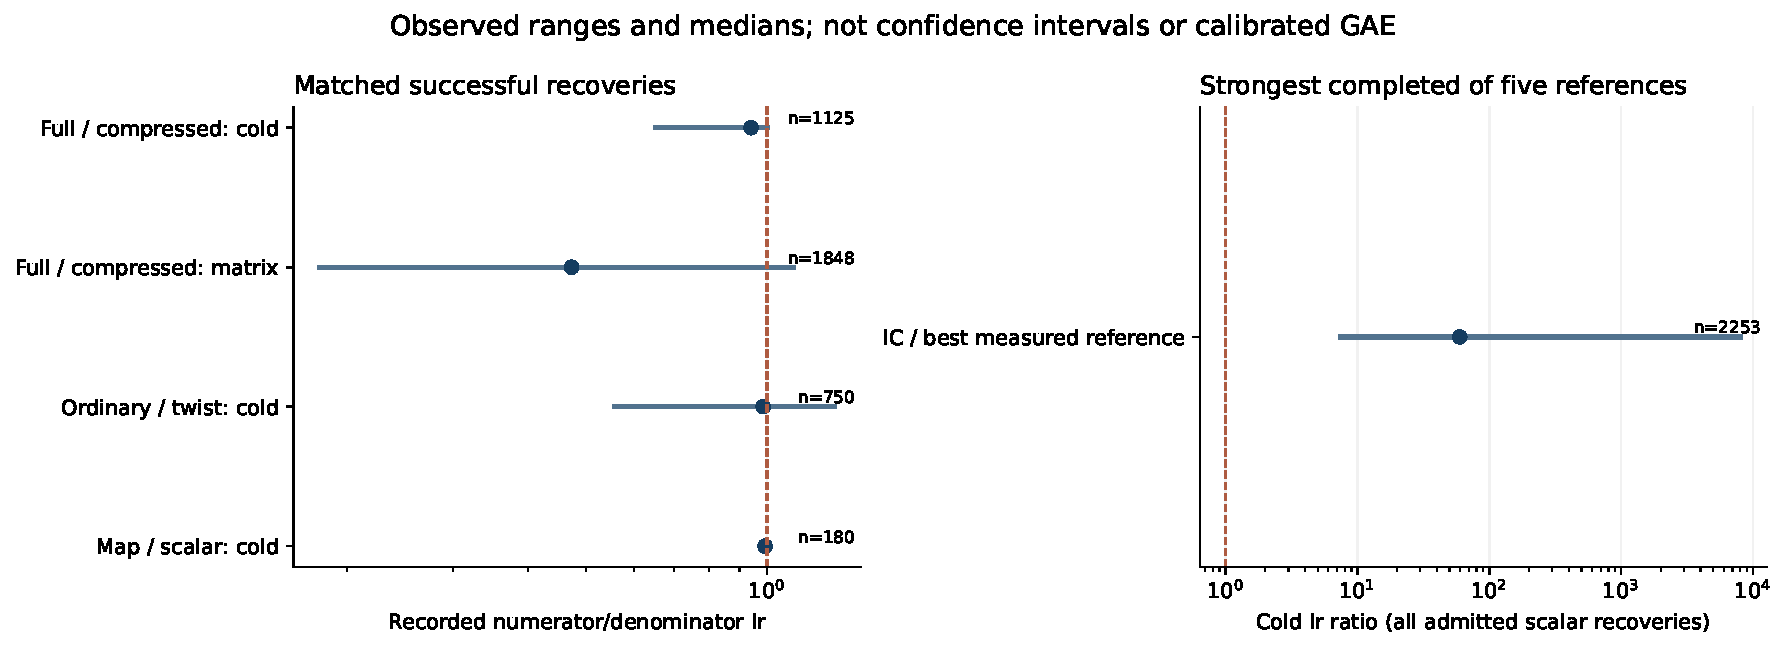
\includegraphics{RATIOS.pdf}
\caption{Native recorded ratio ranges}
\end{figure}

Sources: \href{../../execution-v17/PROTOCOL.md}{frozen protocol},
\href{../../execution-v17/analysis-v2/.artifacts.json}{native data
manifest}, \href{../../execution-v17/FROZEN.json}{source/byte pins}.
\href{../../execution-v17/audit-v2/ADMISSION.json}{Independent GP
admission},
\href{../../execution-v17/ANALYSIS_CORRECTION_V2.json}{reporting
correction}.

Reproduction and raw-object manifests are linked from the evidence
directory. The user-confirmed store is
\texttt{setec-astronomy-artifacts}, region us-east-2. No NIST,
asymptotic, novelty or calibrated-GAE result is established.

\end{document}
